\documentclass{beamer}

\mode<presentation> {
%\usetheme{default}
%\usetheme{AnnArbor}
%\usetheme{Antibes}
%\usetheme{Bergen}
%\usetheme{Berkeley}
%\usetheme{Berlin}
%\usetheme{Boadilla}
%\usetheme{CambridgeUS}
%\usetheme{Copenhagen}
%\usetheme{Darmstadt}
%\usetheme{Dresden}
%\usetheme{Frankfurt}
%\usetheme{Goettingen}
%\usetheme{Hannover}
%\usetheme{Ilmenau}
%\usetheme{JuanLesPins}
%\usetheme{Luebeck}
\usetheme{Madrid}
%\usetheme{Malmoe}
%\usetheme{Marburg}
%\usetheme{Montpellier}
%\usetheme{PaloAlto}
%\usetheme{Pittsburgh}
%\usetheme{Rochester}
%\usetheme{Singapore}
%\usetheme{Szeged}
%\usetheme{Warsaw}

%\usecolortheme{albatross}
%\usecolortheme{beaver}
%\usecolortheme{beetle}
%\usecolortheme{crane}
%\usecolortheme{dolphin}
%\usecolortheme{dove}
%\usecolortheme{fly}
%\usecolortheme{lily}
%\usecolortheme{orchid}
%\usecolortheme{rose}
%\usecolortheme{seagull}
%\usecolortheme{seahorse}
%\usecolortheme{whale}
%\usecolortheme{wolverine}
%\setbeamertemplate{footline} % To remove the footer line in all slides uncomment this line
%\setbeamertemplate{footline}[page number] % To replace the footer line in all slides with a simple slide count uncomment this line

%\setbeamertemplate{navigation symbols}{} % To remove the navigation symbols from the bottom of all slides uncomment this line
}

\usepackage{graphicx} % Allows including images
\usepackage{booktabs} % Allows the use of \toprule, \midrule and \bottomrule in tables


\setbeamertemplate{headline}{%
\leavevmode%
  \hbox{%
    \begin{beamercolorbox}[wd=\paperwidth,ht=2.5ex,dp=1.125ex]{palette quaternary}%
    \insertsectionnavigationhorizontal{\paperwidth}{}{\hskip0pt plus1filll}
    \end{beamercolorbox}%
  }
}

%----------------------------------------------------------------------------------------
%	TITLE PAGE
%----------------------------------------------------------------------------------------

\title[Visual Aid for Blind]{Visual Aid for Blind} % The short title appears at the bottom of every slide, the full title is only on the title page

\author{Niyas P} % Your name

\institute[College of Engineering, Trivandrum] % Your institution as it will appear on the bottom of every slide, may be shorthand to save space
{TVE17ECSP10\\M. Tech (Signal Procesing)\\Third Semester\\
 % Your institution for the title page
\medskip
\textit{https://github.com/niyaspcet/MTechMainProject}\\ % Your email address
\vspace{1cm}
\textit{Guide}\\
Dr. Sreelatha G.\\
Assistant Professor\\
Department of ECE\\
College of Engineering, Trivandrum


}
\date{\today} % Date, can be changed to a custom date
\setbeamertemplate{bibliography item}[text]
\begin{document}

\begin{frame}[plain]

\titlepage % Print the title page as the first slide
\end{frame}

\begin{frame}
\frametitle{Overview} % Table of contents slide, comment this block out to remove it
\tableofcontents % Throughout your presentation, if you choose to use \section{} and \subsection{} commands, these will automatically be printed on this slide as an overview of your presentation
\end{frame}

%----------------------------------------------------------------------------------------
%	PRESENTATION SLIDES
%----------------------------------------------------------------------------------------

%------------------------------------------------
\section{Introduction} % Sections can be created in order to organize your presentation into discrete blocks, all sections and subsections are automatically printed in the table of contents as an overview of the talk
%------------------------------------------------


\begin{frame}
\frametitle{Introduction}
\begin{itemize}
\item
Vision plays a vital role in gaining knowledge of the surrounding
world.
\item
According to the WHO
\begin{itemize}
\item
There are 285 million people in the world with visual
impairment.
\item
39 million of whom are blind
\end{itemize}
\item
Several systems were designed to improve the quality of life of VI (Visually Impaired) people.
\item
White cane and guide dogs were used traditionally
\item
Electronic aids are used nowadays
\item
ETA (Electronic Travel Aids) is an example of such sytem
\end{itemize}
\end{frame}

%------------------------------------------------

\section{Motivation}
\begin{frame}
\frametitle{Motivation}
\begin{itemize}
\item
90\% of VI people lives in developing countries like india
\item
Improving the quality of life of such people is one of the challenging task
\item
Even though there were different travel aids, the acceptance of visual aids are quite low among VI impaired people, which implies further researches.
\end{itemize}
\end{frame}

\section{Objectives}
\begin{frame}
\frametitle{Objectives}
\begin{itemize}
\item
Develop a visual aid which helps visual impaired or low vision people0  with following features.
\begin{itemize}
\item
Navigation
\item
People and object identification
\item
Reading
\end{itemize}
\end{itemize}
\end{frame}


\section{Block Diagram}
\begin{frame}
\frametitle{Block Diagram}
\begin{figure}
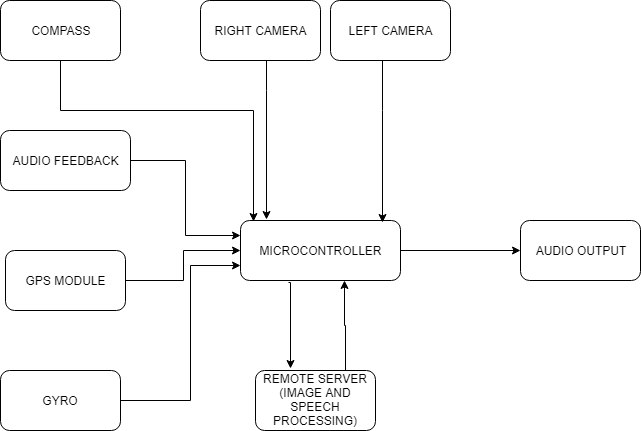
\includegraphics[scale=.45]{block.png}
\end{figure}
\end{frame}


\section{Reference}
\begin{frame}[allowframebreaks]
\frametitle{References}
\bibliography{Bibl}
%\bibliographystyle{IEEETran}
%\scriptsize{\bibliographystyle{acm}}
\scriptsize{\bibliographystyle{IEEETran}}
\nocite{*}
\end{frame}

%------------------------------------------------
\section{Questions}
\begin{frame}
\Huge{\centerline{Questions ?}}
\end{frame}
\begin{frame}
\Huge{\centerline{Thank You}}
\end{frame}

%----------------------------------------------------------------------------------------

\end{document}